\chapter{TD1: Structuration}

L'objectif de ce TD était de s'initier au ``\textit{parsing}'' en Perl. Nous avions un peu plus de 300 pages HTML contenant toute un article issu d'un même site scientifique. Il nous fallait extraire des données ``uniques'' comme le numéro de l'article ou sa rubrique, et des données présentes une (parfois zéro) ou plusieurs fois, comme les paragraphes du texte principal ou les images présentes.

\section{Méthodologie employée}

Pour la totalité des éléments à récupérer, nous avons utilisé des \textit{regex} (sauf pour le nom du fichier que nous récupérerions dans \lstinline{$ARGV}).

Pour produire notre XML, nous avons décidé de tout afficher sur la sortie standard. Il s'agira ensuite de rédiriger cette sortie standard dans un fichier grâce à l'opérateur \lstinline{>} d'Unix.

\subsection{Repérer un élémént d'intérêt}

Pour chaque élément unique qu'il nous fallait récupérer, nous avons essayer de trouver la structure de balises HTML voisinante la plus proche possible qui soit unique. Pour cela, nous avons beaucoup fait appel à la structure \lstinline{.*?} (n'importe quel caractère zéro, une ou plusieurs fois) dans son mode \textit{lazy}. Par exemple, pour le numéro, la structure HTML autour était suffisant simple pour ne pas utiliser ``n'importe quel caractère'' :

\perl
\begin{lstlisting}
$body=~/<span class="style95" style="color:inherit">(\d+)<\/span><\/a>/;
\end{lstlisting}

Tandis que nous en avons eu besoin pour la partie contact :

\begin{lstlisting}
$body =~ /Pour en savoir plus, contacts :.*?<p class="style44"><span class="style85">(.*?)<\/span>/s;
\end{lstlisting}

\subsection{Lecture du contenu d'un fichier}

Nous avons été capables de récuperer le contenu d'un fichier passé en argument grâce à une boucle sur l'opérateur ``diamant''. Fondalement, cet opérateur permet de boucler sur chaque ligne de ``l'\textit{input}''. Nous avons donc simplement récupéré chaque ligne du fichier et avons concaténé ces lignes à une variable \lstinline{$body} initialisée à une chaîne de caractères vide.

\subsection{Lecture du contenu de plusieurs fichiers}

Pour pouvoir récupérer toutes les lignes de chaque fichier tout en dissociant les fichiers, nous avons du opter pour une technique légèrement différente.

\begin{enumerate}
  \item Nous créons une tableau.
  \item Chaque ``case'' du tableau sera une variable similaire à \lstinline{$body} dont nous avons parlé au-dessus: elle contiendra toutes les lignes \textbf{d'un seul fichier}.
  \item Grâce à l'opérateur diamant, nous bouclons sur toutes les lignes de l'\textit{input}.
  \item Nous sommes capable de savoir à tout instant quel fichier nous sommes en train de lire grâce à la variable \lstinline{$ARGV}.
  \item Une fois que nous avons récupéré tous les différents documents dans chaque case du tableau, nous commençons à boucler sur ce tableau de la même manière que nous le faisions pour un seul fichier.
\end{enumerate}

\perl
\begin{lstlisting}
@htmls;
while (<>) {
  $fichier = $ARGV;
  $fichier=~s/.*\///g;
  if (!defined(@htmls{$fichier})) {
    $htmls{$fichier} = $_;
  }
  else {
    $htmls{$fichier} .= $_;
  }
}

print "<corpus>\n";
while (($fichier,$html) = each(%htmls)) {
  print "<bulletin>\n";
  ...
  print "</bulletin>\n";
  }
print "</corpus>\n";
\end{lstlisting}

\section{Commandes Unix}

\subsection{Génération du XML}

Voici la commande Unix utilisée pour récupérer la sortie standard de notre programme et la rediriger dans un fichier XML. Il faut également préciser que nous avons rendu notre programme exécutable grâce à \lstinline{chmod}. De plus, nous utilisons le script \lstinline{convert.pl} pour convertir les entités HTML en caractère Unicode.

\fakeshell
\begin{lstlisting}
./td1.pl BULLETINS/*.htm | perl convert.pl > output.xml
\end{lstlisting}

\subsection{Vérification du nombre d'images}

Nous avons également utilisé quelques commandes Unix supplémentaires dans le but de vérifier que nous récupérerions bien le nombre exactes d'images présentes dans les articles. Par exemple, nous avons utilisé \lstinline{grep} dans son mode \textit{regex}.

\begin{lstlisting}
./td1.pl BULLETINS/*.htm | perl convert.pl > output.xml && { grep "<image>" output.xml } | wc -l && echo "Images parsées en Perl" && { grep -aoE "streaming.+?\.jpg" BULLETINS/*.htm && grep -aoE "<img.*?www\.bulletins-electroniques\.com\/Resources_fm\/actualites.*?\.jpg" BULLETINS/*.htm } | wc -l && echo "Images dans les fichiers d'origine";
\end{lstlisting}

\begin{figure}[H]
  \centering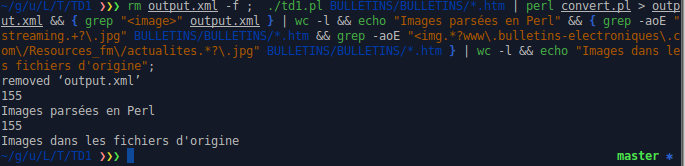
\includegraphics[width=1.00\textwidth]{images/output_td1.png}
  \caption{Résultat de la commande}
\end{figure}

% pour l'index, parler de la granularité (bulletin, article) (question 1.1)
